\documentclass[conference]{IEEEtran}
\usepackage{amsmath,amssymb,graphicx,booktabs,array,url}
\usepackage[hidelinks]{hyperref}
\usepackage{cite}
\newcommand{\AURA}{\textsc{Aura}}
\title{AURA: Assessing the Limits of Disagreement-Aware Selective Prediction in an Axial Spondyloarthritis-Inspired Synthetic Benchmark}
\author{\IEEEauthorblockN{Anonymous author(s)}\IEEEauthorblockA{Author details withheld for review}}
\begin{document}
\maketitle
\begin{abstract}
Inter-modality disagreement is often proposed as an uncertainty signal for selective prediction, but its incremental value beyond confidence and evidence quality is not guaranteed. We investigate this question using AURA, a lightweight reliability-weighted fusion test bed, in an axial spondyloarthritis (axSpA)-inspired synthetic benchmark. Ten independent simulation seeds, seven observation or population conditions and six classifiers are evaluated under matched ranking protocols; additional native AURA ablations and nine sensitivity settings isolate the role of disagreement. Relative to equal fusion, learned fusion improves AUROC by 0.00251 (95\% paired seed-level interval [0.00200, 0.00302]) and Brier score by $-0.00150$ ([$-0.00178,-0.00122$]). A native learned ranker reduces area under the risk-coverage curve (AURC) relative to entropy by $-0.00424$ ([$-0.00568,-0.00280$]), but adding disagreement yields $-0.00014$ ([$-0.00069,0.00042$]); all nine sensitivity intervals span zero. Early logistic regression retains the lowest mean AURC under shared ranking protocols. These results constrain the methodological claim that disagreement is independently useful: neither its benefit nor its absence in other settings is established. All data are simulated, with illustrative rather than clinically calibrated parameters. The study evaluates algorithmic behavior in this generator, not axSpA diagnostic performance, clinical evidence relationships or readiness.
\end{abstract}
\begin{IEEEkeywords}
selective prediction, multimodal fusion, missing modalities, simulation, uncertainty ranking, attribution stability, negative results
\end{IEEEkeywords}
\section{Introduction}
Axial spondyloarthritis is an inflammatory rheumatic condition affecting the axial skeleton. Its assessment incorporates patient history, laboratory findings and imaging of the sacroiliac joints. Clinical guidance emphasizes that negative HLA-B27 and normal inflammatory markers cannot independently exclude disease \cite{nice}. Furthermore, imaging findings can overlap with non-inflammatory conditions and classification criteria should not be treated as a diagnostic reference standard \cite{mri,asas}. These properties motivate decision-support research that explicitly represents incomplete and potentially inconsistent evidence.

Machine learning (ML) has been studied in axSpA for both imaging interpretation and clinical prediction \cite{adams,meta}. Recent diagnostic systems combine imaging and risk features, including multicenter deep learning \cite{xie}, conventional random forests \cite{rf}, TabNet \cite{tabnet} and explainable segmentation-assisted decision support \cite{cdss}. Accordingly, neither multimodal integration nor interpretability alone constitutes a novel technical claim. More generally, quality-aware fusion and cross-view conflict modelling are established directions in multimodal learning \cite{tmc,qamoe,aemrl}.

A related problem concerns \emph{selective prediction}: a model may defer a decision rather than output an uncertain classification. The important question is whether a proposed uncertainty statistic identifies errors more effectively than confidence alone, especially in the presence of incomplete data. Agreement between individually unreliable sources does not guarantee correctness; conversely, disagreement may represent useful complementary evidence rather than error. This motivates a matched comparison that holds predicted probabilities constant while varying the error-ranking features.

This study uses AURA as an auditable test bed rather than claiming a novel state-of-the-art architecture. Its contribution is an investigation of the limits of a methodological claim: (i) a reproducible axSpA-inspired synthetic stress benchmark; (ii) matched classifier and ranking comparisons that separate the effects of fusion from the incremental effect of dispersion; (iii) paired uncertainty intervals, sensitivity analyses and held-out permutation diagnostics; and (iv) algebraically checked and cross-seed tested model attributions. A negative result is informative precisely because a plausible mechanism need not improve selective prediction. The simulated binary class is not an independently adjudicated clinical diagnosis.
\section{Related Work and Research Gap}
\subsection{AxSpA clinical and imaging models}
A clinical diagnostic review describes the limitations of isolated laboratory and imaging findings \cite{clinical}. A meta-analysis examines AI tools across radiography, CT and MRI \cite{meta}. Xie et al. combine 3D MRI representations with clinical predictors in a four-center cohort of 1,294 patients \cite{xie}. A rheumatological routine-care study uses random forests and imputation on 939 records \cite{rf}. TabNet combines structured SIJ findings with clinical variables in 942 patients \cite{tabnet}; MRI and clinical models have also been investigated in HLA-B27-negative disease \cite{negative}. A more recent clinical decision support architecture combines multi-sequence MRI with risk scores and segmentation-based interpretation \cite{cdss}. These studies motivate the feature groups, but their reported clinical discrimination cannot be compared directly with results from generated records.
\subsection{Missingness, reliability and selective prediction}
Multimodal learning taxonomies distinguish representation, fusion and alignment \cite{bal}. Modality dropout and heterogeneous modality aggregation offer approaches to unavailable inputs \cite{moddrop,hemis}. Clinical multimodal robustness remains an active area, including attention-based fusion \cite{attention} and a recent mechanism-level review \cite{missingreview}. Trusted multi-view classification uses dynamic evidential fusion \cite{tmc}; multimodal dynamics estimates sample-specific informativeness \cite{dynamics}. QA-MoE integrates quality scoring, stable subset selection and expert routing, including abstaining experts \cite{qamoe}. Conflict-aware calibration has likewise been investigated \cite{aemrl}. These methods are important conceptual competitors, but this paper does not claim to reproduce or outperform their original implementations.

Reject-option classification and risk-coverage evaluation are established \cite{selective}. Calibration \cite{guo}, ensemble-based uncertainty \cite{ensembles} and robustness under dataset shift \cite{ovadia} inform the evaluation. Recent multimodal clinical selective prediction work highlights failure modes caused by calibration and class imbalance \cite{lopez}. We therefore distinguish class-probability calibration from error-ranking performance and report both coverage-matched and fixed-threshold outcomes.
\begin{table}[t]
\caption{Closest conceptual comparators (not matched-data results).}
\label{tab:related}
\centering\footnotesize
\begin{tabular}{@{}p{0.19\columnwidth}p{0.34\columnwidth}p{0.36\columnwidth}@{}}\toprule
Work & Established contribution & Distinction in this study\\\midrule
Xie et al. \cite{xie} & MRI + clinical predictors & Synthetic evidence stress tests\\
TabNet \cite{tabnet} & Structured MRI + risk & Matched selective ranking\\
CDSS \cite{cdss} & MRI + explainable segmentation & Coalition explanations, no raw MRI\\
TMC \cite{tmc} & Dynamic evidential fusion & Lightweight inverse-error gate\\
QA-MoE \cite{qamoe} & Quality-aware expert selection & Explicit disagreement-only ablation\\
AEMRL \cite{aemrl} & Conflict-aware calibration & Test whether disagreement adds value\\
Lopez et al. \cite{lopez} & Clinical selective prediction & Binary synthetic axSpA-inspired task\\\bottomrule
\end{tabular}
\end{table}
\subsection{Scope of the gap}
Table~\ref{tab:related} summarizes the nearest methodological and clinical precedents identified in a targeted scoping search. The associated research matrix records 44 publications/resources across clinical diagnosis, axSpA AI, data access, fusion, uncertainty, explanation and reporting. Searches used combinations of axSpA/ankylosing spondylitis, diagnosis, MRI, missing modality, clinical prediction, conflict, calibration and selective classification, with foundational papers retained irrespective of publication year. The matrix is based on metadata, abstracts and selected accessible full-text material; it is not an exhaustive systematic review. We do not claim that no prior study has tested disagreement. Our specific question is whether weighted prediction dispersion adds incremental error-ranking value on an explicit axSpA-inspired stress benchmark after controlling for confidence, availability and quality.
\section{Problem Formulation}
Let $Y\in\{0,1\}$ be a latent simulated class and $X=(X_C,X_L,X_I)$ represent clinical, laboratory and structured imaging evidence. Let $m_k\in\{0,1\}$ indicate modality availability and $q_k\in[0,1]$ denote an observed quality proxy for $k\in\{C,L,I\}$. The objective is to estimate a class probability $\hat p$ and an error-ranking score $u$ for records with at least one available modality. The selective classifier is
\begin{equation}
 h_\tau(X,m,q)=\begin{cases}\bot,&\sum_km_k=0\ \text{or}\ u>\tau,\\\mathbb{1}[\hat p\geq 0.5],&\text{otherwise}.\end{cases}
\end{equation}
Here $\bot$ represents deferral, not a negative class. The implementation evaluates nonempty masks only; an operational system would have to handle zero evidence explicitly. The threshold 0.5 is a computational convention, not a clinical referral cutoff.

For error indicator $e_i=\mathbb{1}[\hat y_i\neq y_i]$, coverage $c(\tau)$ and selective risk $r(\tau)$ are
\begin{align}
c(\tau)&=n^{-1}\sum_i\mathbb{1}[u_i\leq\tau],\\
r(\tau)&=\frac{\sum_i e_i\mathbb{1}[u_i\leq\tau]}{\sum_i\mathbb{1}[u_i\leq\tau]},
\end{align}
where risk is undefined at zero coverage. AURC is calculated empirically by sorting records from lowest to highest error score and averaging cumulative error over all retained-set sizes. Specifically, $\mathrm{AURC}=n^{-1}\sum_{j=1}^{n}j^{-1}\sum_{i=1}^{j}e_{(i)}$, where parentheses denote increasing error-score order. Exact ties use the expected cumulative error under uniformly random within-tie ordering: each tied observation contributes the mean error of its tie block. Lower AURC means better selective performance, conditional on the underlying classifier. Fixed-coverage risk $R_{80}$ is the cumulative risk at $\lfloor0.8n\rfloor$ retained observations (same tie convention). It is distinct from risk at a fixed score cutoff.

Three questions guide evaluation: RQ1: Does learned fusion improve discrimination/calibration relative to equal and observed-quality weighting? RQ2: Does learned error ranking improve AURC relative to entropy? RQ3 (primary comparison): Does disagreement improve AURC relative to an otherwise identical ranker? The analysis is exploratory, not prospectively preregistered.
\section{AURA Test Bed and Ranking Protocols}
\subsection{Modality experts and reliability gate}
For each modality, five logistic regression models are fit on independent bootstrap resamples of the expert-training partition, using standardized features and quality. Their mean and variance are
\begin{align}
p_k &= B^{-1}\sum_{b=1}^{B}p_{kb},\quad B=5,\\
v_k &= B^{-1}\sum_{b=1}^{B}(p_{kb}-p_k)^2.
\end{align}
Variance is a heuristic measure of model instability, not a full Bayesian decomposition. Using a disjoint gate partition, ridge regression estimates the squared probability error $\ell_k=\bigl(p_k-Y\bigr)^2$ from $z_k=[q_k,|p_k-0.5|,q_k|p_k-0.5|,q_k^2]$. For the fitted estimate $g_k(z_k)$, define
\begin{align}
a_k&=\{\max(0.03,g_k(z_k))\}^{-1},\\
w_k&=\frac{m_ka_k}{\sum_j m_ja_j},\qquad p_f=\sum_kw_kp_k.
\end{align}
The gate uses ridge regularization $\alpha=5$. The inverse predicted error is a transparent heuristic: for independent, unbiased estimators with known error variances, inverse-variance weighting minimizes the variance of a weighted mean. Here errors may be biased and correlated, so that optimality argument does not apply; the gate is evaluated empirically. Clipping prevents arbitrarily large weights. Missing inputs receive zero weight. Equal and quality-weighted fusion use the identical experts but replace $a_k$ with 1 and $q_k$, respectively.
\subsection{Calibration and disagreement}
A separate calibration partition fits a logistic recalibrator
\begin{equation}
\hat p=\sigma(b_0+b_1\operatorname{logit}(\operatorname{clip}(p_f))),
\end{equation}
where probability clipping uses $10^{-6}$ and $1-10^{-6}$. All comparator probability outputs receive the same type of recalibration. This avoids conflating the choice of fusion with the presence of calibration.

Disagreement is the weighted dispersion of expert means,
\begin{equation}
D=\sum_kw_k(p_k-p_f)^2=\sum_kw_kp_k^2-p_f^2.
\end{equation}
Since each $p_k\in[0,1]$, $0\leq D\leq1/4$; thus $4D\in[0,1]$. A single available modality has $D=0$, which does not imply high reliability. Two models that make similarly erroneous predictions also produce low disagreement. These cases motivate the inclusion of other uncertainty features.
\subsection{Matched error ranking}
On the dedicated uncertainty-development partition, fit standardized logistic regressions to predict $e=\mathbb{1}[\mathbb{1}[\hat p\geq0.5]\neq Y]$. The baseline feature vector is
\begin{equation}
 t_0=[H_2(\hat p),\sum_kw_kv_k,\tfrac{1}{3}\sum_km_k,\bar q,m_C,m_L,m_I],
\end{equation}
where $H_2$ is binary entropy in bits and $\bar q=\sum_k m_k q_k/\sum_km_k$. The native full ranker adds $4D$ to $t_0$. For fair cross-classifier comparisons, we additionally define a shared-context protocol: the weighted expert variance and $4D$ are computed from the same auxiliary equal-weight expert ensemble for all six classifiers, while entropy is computed from each classifier's own calibrated probability. Availability, quality and mask indicators are identical across classifiers. Each classifier has its own logistic error ranker, fitted on its own error labels on the same development records, with the same standardized features and regularization ($C=1$). Thus all classifiers have access to the same ranking information, including the extra cost of fitting the auxiliary experts. This is a matched training protocol, not a claim that ranker coefficients or predictions are identical across classifiers. Native AURA uses its learned fusion weights for variance and disagreement; its matched ablation remains the primary RQ3 comparison. Both rankers use the same model class, default regularization and data. The entropy-only comparator ranks solely by $H_2$. All three share exactly the same $\hat p$ and class predictions, enabling isolation of ranking effects from classification effects. The fixed operating threshold is the 80th percentile of full-ranker scores on the ranker-development partition; this is an in-sample threshold selection and is not a risk guarantee.
\subsection{Two-level explanation}
For the set $A$ of available modalities, define the coalition value $V(S)$ for $S\subseteq A$ by renormalizing existing weights over $S$ and recalibrating the resulting score. Set $V(\emptyset)$ to the recalibrated score at raw probability 0.5. The exact Shapley contribution \cite{shap} of modality $k$ is
\begin{equation}
\phi_k=\sum_{S\subseteq A\setminus\{k\}}\frac{|S|!(|A|-|S|-1)!}{|A|!}[V(S\cup\{k\})-V(S)].
\end{equation}
With at most three modalities, exact enumeration is feasible. The attributions sum to $V(A)-V(\emptyset)$, but depend on the chosen reference and masking rule. They are model-specific, not causal. For within-modality interpretation, standardized feature contributions $\beta_j z_j$ of the first logistic expert member are reported on its logit scale. This view is exact for that member, not a decomposition of the entire ensemble. The two explanation levels are deliberately not added together.
\begin{figure}[t]
\centering
\setlength{\fboxsep}{3pt}
\begin{tabular}{c}
\fbox{\parbox{.91\columnwidth}{\centering Clinical $\mid$ Laboratory $\mid$ Structured imaging}}\\[-1pt]
$\downarrow$\\
\fbox{\parbox{.91\columnwidth}{\centering Bootstrap experts: $p_k,v_k$; observed $m_k,q_k$}}\\[-1pt]
$\downarrow$\\
\fbox{\parbox{.91\columnwidth}{\centering Ridge error gate $\rightarrow$ masked fusion $\rightarrow$ calibration}}\\[-1pt]
$\downarrow$\\
\fbox{\parbox{.91\columnwidth}{\centering Entropy, variance, quality, mask, disagreement}}\\[-1pt]
$\downarrow$\\
\fbox{\parbox{.91\columnwidth}{\centering Error ranker $\rightarrow$ classify or defer\\ Coalition and expert-logit explanations}}\\
\end{tabular}
\caption{AURA computational architecture. The output is a simulated binary assessment, not a clinical diagnosis.}
\label{fig:arch}
\end{figure}
\section{Synthetic Benchmark and Experimental Protocol}
\subsection{Data provenance and generation}
The DESIR cohort is a potential source of longitudinal diagnostic evidence, but access is subject to request and governance \cite{desir}. No suitable matched open clinical/laboratory/imaging dataset was obtained in the present study. Therefore, all observations are generated by code. The generator is inspired by qualitative clinical evidence, not fitted to patient-level distributions or published diagnostic likelihood ratios. No medical record, raw image, identifiable data or physician diagnosis was used.

For each seed, sample 10,000 latent labels $Y\sim\operatorname{Bernoulli}(0.40)$ and an inflammation proxy $Z\sim\mathcal N(0.8Y,1)$. A latent mimic indicator $J$ is sampled with probability 0.17 for negative cases and 0.08 for positives, creating shared non-specific evidence. Let $G\sim\mathcal N(0,1)$ be a second latent factor. Binary observations follow $X_j\sim\operatorname{Bernoulli}(\sigma(a_j+b_jY+c_jZ+d_jJ+e_jG))$; continuous proxies are affine combinations of the latent variables with unit Gaussian noise. Table~\ref{tab:coeff} specifies the clean generator. The label is sampled before features; it is not the output of a clinical classification rule or of AURA. Nevertheless, the chosen causal structure can favor certain learners and is not claimed to reproduce disease mechanisms.
\begin{table}[t]
\caption{Synthetic feature generator coefficients. B = Bernoulli with logistic link; N = Gaussian with unit variance.}
\label{tab:coeff}
\centering\footnotesize
\begin{tabular}{@{}llrrrrr@{}}\toprule
Feature & Type & $a$ & $b$ & $c$ & $d$ & $e$\\\midrule
Stiffness & B & -.9 & 1.1 & .55 & .8 & 0\\
Movement relief & B & -.9 & 1.5 & .3 & .3 & 0\\
Night pain & B & -1 & 1.1 & .5 & .7 & 0\\
Extra-articular & B & -2 & 1.35 & 0 & 0 & .2\\
HLA-B27 & B & $-2.2$ & 2.15 & 0 & 0 & .3\\
CRP proxy & N & 0 & .55 & .48 & .22 & 0\\
ESR proxy & N & 0 & .35 & .52 & .22 & 0\\
BME & B & -1.8 & 1.65 & .65 & 1.9 & 0\\
Erosion & B & -2.2 & 1.8 & .42 & .35 & 0\\
Structural proxy & N & 0 & .55 & .35 & .45 & 0\\\bottomrule
\end{tabular}
\end{table}

Quality $q_k$ is independently sampled from $\mathrm{Beta}(5,2)$ under the reference acquisition mechanism. For each binary feature, its clean value is flipped with probability $0.36(1-q_k)$; continuous features receive independent zero-mean Gaussian perturbations with standard deviation $1.2(1-q_k)$. CRP, ESR and structural features are dimensionless proxies, not clinically interpretable laboratory or radiology measurements. The latent mimic flag is excluded from model inputs. Quality is an observed simulator variable; in clinical practice an independently validated quality estimator would be required.
\subsection{Stress conditions}
\begin{table}[t]
\caption{Seven evaluation conditions; masks with zero modalities are repaired by uniformly selecting one modality.}
\label{tab:scen}
\centering\footnotesize
\begin{tabular}{@{}p{.26\columnwidth}p{.67\columnwidth}@{}}\toprule
Condition & Observation/population intervention\\\midrule
Complete & All three modalities, reference quality\\
MCAR30 & Independent pre-repair dropout 30\%\\
MCAR50 & Independent pre-repair dropout 50\%\\
Quality & $q_k\sim\mathrm{Beta}(2,4)$; more observation noise\\
Selective & Lab/MRI acquisition depends on symptoms and latent class\\
Mimic & Prevalence 25\%, negative mimic rate 48\%\\
Combined & Mimic population, low quality, 40\% dropout\\\bottomrule
\end{tabular}
\end{table}
Table~\ref{tab:scen} summarizes stress conditions. For selective acquisition, clinical evidence is always present and the laboratory and imaging acquisition probabilities are $\sigma(-0.7+1.15X_1+0.55Y)$ and $\sigma(-1.1+1.4X_2+0.7Y)$, respectively, using clean clinical indicators. Dependence on unobserved $Y$ intentionally creates missing-not-at-random (MNAR) stress. In the mimic and combined conditions, new independent populations are sampled with positive prevalence 0.25 and negative mimic probability 0.48; all other generator coefficients remain fixed. This is not a validated model of specific infectious, mechanical or degenerative diagnoses. Conditions sharing the reference population reuse the same held-out records but sample independent observation perturbations. For every condition, at least one modality is retained; nominal dropout rates therefore differ from realized missingness. In the Quality and Combined conditions, drawing lower $q_k$ also increases the observation corruption via the same noise equations, rather than merely changing a metadata input. Repair of all-zero masks is a simulator design choice that conditions the evaluated problem on nonempty evidence, not a realistic acquisition or deferral policy; no inference is made about entirely missing records.
\subsection{Data splitting, comparators and metrics}
Ten seeds (20261124 through 20261133) are run independently. Each reference population is partitioned into 5,000 expert-training, 1,500 gate, 1,000 calibration, 1,000 ranker-development and 1,500 held-out records. Training, gate, calibration and ranker observations use reference quality and nominal 22\% dropout (experts are trained using available generated measurements before masking). The shifted evaluation populations contain 1,500 new observations per seed and condition. Model fitting never uses test labels. The experiment uses the same partitions and observed test features for every configuration within each seed and condition.

Six classifiers are evaluated: mask-aware early logistic regression, random forest (80 trees, minimum leaf size 8), histogram gradient boosting (100 iterations, at most 15 leaves), equal late fusion, quality late fusion, and learned AURA fusion. Early fusion concatenates zero-filled features, mask indicators and masked quality. All six receive dedicated probability recalibration. Each is evaluated with entropy, a shared-context ranker without $D$, and a shared-context ranker with $D$; AURA additionally receives two native rankers (20 configurations, 1,400 seed-condition-configuration evaluations). The same expert predictions, acquired observations and partitions are retained from the initial benchmark. No hyperparameter selection is made using test data.

We calculate AUROC, area under the precision-recall curve as average precision (AUPRC), Brier score, log loss, accuracy, ten-bin equal-width expected calibration error (ECE), AURC, fixed-coverage selective risk, and error-detection AUROC. Macro means weight each condition equally, then each seed equally. Paired contrasts first average the seven condition-level differences within each seed, then use a two-sided Student-$t$ interval with nine degrees of freedom across ten seed means. These intervals reflect variability under the stipulated simulator, not clinical uncertainty. Secondary comparisons are exploratory and unadjusted for multiplicity. Fixed thresholds are estimated only on the ranker-development partition; ties at the threshold are retained.

Sensitivity analyses vary one factor at a time around the default: bootstrap members $B\in\{3,5,10\}$, lower gate clipping $\in\{0.01,0.03,0.10\}$, ridge $\alpha\in\{1,5,20\}$, and ranker inverse regularization $C\in\{0.1,1,10\}$. The nine configurations reuse identical observations and partitions and nested bootstrap members; all gate, calibration and ranker fits are recomputed as appropriate. For the default native ranker we report standardized $4D$ coefficients and odds ratios per development standard deviation. In each held-out condition, $4D$ is shuffled ten times with fixed ranker and class probabilities; we report increases in AURC and decreases in error AUROC. Marginal permutation can disrupt feature dependencies, so this is a diagnostic, not a causal or conditional importance estimate. Individual experts are separately recalibrated on available calibration records and evaluated on available test records. For attribution stability, 150 independent complete-condition anchor records (fixed across seeds) are passed through all ten fitted default systems. All 45 seed pairs are compared for absolute attribution difference, sign agreement and agreement on the largest absolute attribution. The pairs are dependent; their means are descriptive, not 45 independent samples.
\section{Results}
\subsection{RQ1: Fusion performance}
\begin{table}[t]
\caption{Class probability performance (identical across ranking rules). Bold indicates the best macro mean, not a significance claim.}
\label{tab:macro}
\centering\footnotesize
\begin{tabular}{@{}lrrrr@{}}\toprule
Classifier & AUROC & AUPRC & Brier & ECE\\\midrule
Early logistic & \textbf{0.8296} & \textbf{0.7330} & \textbf{0.1594} & \textbf{0.0631}\\
Early RF & 0.8185 & 0.7154 & 0.1655 & 0.0694\\
Early HGB & 0.8184 & 0.7151 & 0.1645 & 0.0640\\
Equal fusion & 0.8246 & 0.7144 & 0.1629 & 0.0687\\
Quality fusion & 0.8249 & 0.7150 & 0.1628 & 0.0683\\
AURA & 0.8271 & 0.7192 & 0.1614 & 0.0648\\\bottomrule
\end{tabular}
\end{table}
\begin{table}[t]
\caption{RQ1: AURA minus comparator; paired 95\% seed-level intervals (unadjusted).}
\label{tab:fusionci}
\centering\footnotesize
\begin{tabular}{@{}llrl@{}}\toprule
Comparator & Metric & $\Delta$ & 95\% interval\\\midrule
Equal fusion & AUROC & 0.00251 & [0.00200, 0.00302]\\
 & AUPRC & 0.00486 & [0.00381, 0.00590]\\
 & BRIER & -0.00150 & [-0.00178, -0.00122]\\
 & ECE & -0.00392 & [-0.00551, -0.00233]\\
Quality fusion & AUROC & 0.00218 & [0.00128, 0.00309]\\
 & AUPRC & 0.00422 & [0.00284, 0.00561]\\
 & BRIER & -0.00144 & [-0.00189, -0.00099]\\
 & ECE & -0.00351 & [-0.00553, -0.00150]\\\bottomrule
\end{tabular}
\end{table}
Table~\ref{tab:macro} reports probability metrics independently of ranking. Learned fusion yields higher AUROC and AUPRC and lower Brier and ECE than equal and quality weighting; the paired seed-level intervals in Table~\ref{tab:fusionci} exclude zero for all eight contrasts, although gains are small and intervals are not multiplicity-adjusted. Early logistic regression has the highest mean AUROC and AUPRC and lowest Brier; AURA minus early logistic AUROC is $-0.00254$ (95\% interval [$-0.00427,-0.00081$]), AUPRC $-0.01372$ ([$-0.01736,-0.01009$]), and Brier $+0.00199$ ([0.00087, 0.00310]). ECE difference $+0.00173$ ([$-0.00128,0.00475$]) is inconclusive. These are simulator-specific effects, not medical performance estimates.
\subsection{RQ2: Matched ranking comparisons}
\begin{table}[t]
\caption{AURC by classifier and shared ranking protocol. Columns compare classifiers under the same feature definitions. Lower is better; column minima in bold.}
\label{tab:rank}
\centering\footnotesize
\begin{tabular}{@{}lrrr@{}}\toprule
Classifier & Entropy & No $D$ & With $D$\\\midrule
Early logistic & \textbf{0.1193} & \textbf{0.1197} & \textbf{0.1200}\\
Early RF & 0.1306 & 0.1320 & 0.1311\\
Early HGB & 0.1295 & 0.1297 & 0.1293\\
Equal fusion & 0.1281 & 0.1233 & 0.1235\\
Quality fusion & 0.1280 & 0.1231 & 0.1237\\
AURA & 0.1260 & 0.1220 & 0.1219\\\bottomrule
\end{tabular}
\end{table}
\begin{table}[t]
\caption{Within-classifier ranking contrasts in AURC. H = entropy. Shared features; unadjusted 95\% intervals.}
\label{tab:rankci}
\centering\footnotesize
\begin{tabular}{@{}llrl@{}}\toprule
Classifier & Contrast & $\Delta$ & 95\% interval\\\midrule
Early logistic & No $D$--H & 0.00038 & [-0.00040, 0.00117]\\
 & With--no $D$ & 0.00026 & [-0.00015, 0.00067]\\
Early RF & No $D$--H & 0.00139 & [0.00039, 0.00238]\\
 & With--no $D$ & -0.00081 & [-0.00162, -0.00000]\\
Early HGB & No $D$--H & 0.00018 & [-0.00107, 0.00144]\\
 & With--no $D$ & -0.00036 & [-0.00096, 0.00023]\\
Equal fusion & No $D$--H & -0.00483 & [-0.00677, -0.00288]\\
 & With--no $D$ & 0.00028 & [-0.00007, 0.00063]\\
Quality fusion & No $D$--H & -0.00487 & [-0.00657, -0.00317]\\
 & With--no $D$ & 0.00053 & [-0.00017, 0.00122]\\
AURA & No $D$--H & -0.00402 & [-0.00551, -0.00252]\\
 & With--no $D$ & -0.00005 & [-0.00046, 0.00035]\\\bottomrule
\end{tabular}
\end{table}
Under common ranking feature definitions (Table~\ref{tab:rank}), AURA outperforms equal and quality fusion in mean AURC, both with and without $D$. With the full shared ranker, paired AURA-minus-equal and AURA-minus-quality differences are $-0.00162$ ([$-0.00195,-0.00129$]) and $-0.00176$ ([$-0.00271,-0.00081$]). Early logistic has the lowest mean AURC in each column. Under the full shared protocol, AURA minus early logistic is $+0.00193$ ([$-0.00073,0.00459$]); neither superiority nor equivalence is established. Under entropy alone this contrast is $+0.00664$ ([0.00382, 0.00947]). The comparison no longer conflates access to ranking features with the classifier, but separately trained rankers may still differ in their fit. Table~\ref{tab:rankci} isolates ranking effects within each fixed classifier; learned ranking helps all three late-fusion classifiers relative to entropy without $D$, but not uniformly for early fusion. The native AURA learned full ranker improves mean AURC from 0.12598 to 0.12174, a paired difference of $-0.00424$ ([$-0.00568,-0.00280$]).
\begin{figure}[t]
\centering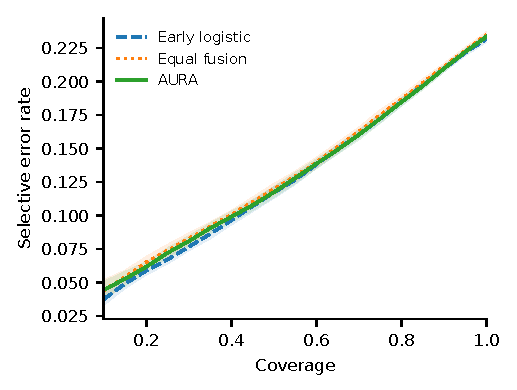
\includegraphics[width=\columnwidth]{revision_figures/risk_coverage.pdf}
\caption{Matched full ranker: macro selective risk, with pointwise 95\% seed-level $t$ bands for selected classifiers. Curves sampled at 0.10--1.00 in 0.05 increments; AURC uses every retained-set size, including exact-tie averaging. Bands are not simultaneous.}
\label{fig:rc}
\end{figure}
\subsection{RQ3: Incremental disagreement and sensitivity}
The primary native ablation holds every class probability and prediction fixed. Adding $4D$ changes AURC from 0.12188 to 0.12174 ($\Delta=-0.000138$, 95\% interval [$-0.000692,0.000415$]); error-detection AUROC changes from 0.7188 to 0.7184. The shared-context AURA ablation likewise yields $-0.000052$ ([$-0.000456,0.000351$]). None of the nine one-factor sensitivity intervals excludes zero (Table~\ref{tab:sens}); their mean effects range from $-0.000313$ to $+0.000029$. The experiments do not establish a useful disagreement gain, nor prove absence of any effect. The early RF shared-context contrast has a small unadjusted negative interval barely excluding zero; it is exploratory and does not establish a general benefit.
\begin{table}[t]
\caption{One-factor-at-a-time sensitivity: native AURA, full minus no-disagreement AURC. All intervals span zero.}
\label{tab:sens}
\centering\footnotesize
\begin{tabular}{@{}lrrrl@{}}\toprule
Setting & No $D$ & Full & $\Delta$ & 95\% interval\\\midrule
default & 0.12188 & 0.12174 & -0.00014 & [-0.00069, 0.00041]\\
B=3 & 0.12195 & 0.12191 & -0.00004 & [-0.00044, 0.00035]\\
B=10 & 0.12194 & 0.12197 & 0.00003 & [-0.00060, 0.00065]\\
clip=.01 & 0.12188 & 0.12174 & -0.00014 & [-0.00069, 0.00041]\\
clip=.10 & 0.12190 & 0.12180 & -0.00010 & [-0.00066, 0.00046]\\
ridge=1 & 0.12232 & 0.12201 & -0.00031 & [-0.00102, 0.00040]\\
ridge=20 & 0.12203 & 0.12204 & 0.00001 & [-0.00033, 0.00036]\\
C=.1 & 0.12169 & 0.12150 & -0.00019 & [-0.00063, 0.00024]\\
C=10 & 0.12192 & 0.12179 & -0.00013 & [-0.00071, 0.00045]\\\bottomrule
\end{tabular}
\end{table}
The native ranker's mean standardized $4D$ coefficient is 0.01551 (95\% interval [$-0.05819,0.08921$]); five of ten coefficients are positive, range $[-0.09884,0.18703]$. The mean of per-seed odds ratios per standard deviation is 1.02060. Held-out marginal permutation increases AURC by 0.000436 ([$-0.000016,0.000887$]) and decreases error-detection AUROC by 0.000948 ([$-0.000384,0.002279$]). Neither interval excludes zero. These diagnostics are consistent with limited incremental ranking value in this generator. They are not independent evidence of clinical importance; the coefficient and permutation analyses share fitted models and generated data.
\subsection{Stress response and threshold transport}
\begin{table}[t]
\caption{Native full AURA: fixed-coverage risk $R_{80}$ uses the lowest-scored 80\% of each test set.}
\label{tab:stress}
\centering\footnotesize
\begin{tabular}{@{}lrrrrr@{}}\toprule
Condition & AUROC & AUPRC & ECE & AURC & $R_{80}$\\\midrule
Complete & 0.8828 & 0.8341 & 0.0472 & 0.0818 & 0.1389\\
MCAR30 & 0.8457 & 0.7800 & 0.0309 & 0.1092 & 0.1717\\
MCAR50 & 0.8159 & 0.7395 & 0.0489 & 0.1340 & 0.1969\\
Quality & 0.8198 & 0.7529 & 0.0304 & 0.1331 & 0.2035\\
Selective & 0.8288 & 0.7519 & 0.0385 & 0.1266 & 0.1912\\
Mimic & 0.8543 & 0.6890 & 0.1139 & 0.0859 & 0.1427\\
Combined & 0.7422 & 0.4873 & 0.1439 & 0.1816 & 0.2440\\\bottomrule
\end{tabular}
\end{table}
\begin{table}[t]
\caption{Development-selected threshold: realized test coverage and conditional error, not fixed 80\% coverage.}
\label{tab:threshold}
\centering\footnotesize
\begin{tabular}{@{}lrr@{}}\toprule
Condition & Coverage & Risk\\\midrule
Complete & 0.8836 & 0.1608\\
MCAR30 & 0.7697 & 0.1643\\
MCAR50 & 0.7166 & 0.1791\\
Quality & 0.7001 & 0.1795\\
Selective & 0.7661 & 0.1816\\
Mimic & 0.8744 & 0.1642\\
Combined & 0.5956 & 0.2031\\\bottomrule
\end{tabular}
\end{table}
The combined condition decreases native AURA AUROC from 0.8828 to 0.7422, AUPRC from 0.8341 to 0.4873 and increases ECE from 0.0472 to 0.1439. AUPRC also depends on prevalence, which changes in the Mimic and Combined conditions. At fixed 80\% test coverage, the native full ranker has macro risk 0.18415 versus 0.18114 for AURA entropy: better integrated risk does not guarantee improvement at every operating point. The development-selected score threshold retains 88.36\% of Complete records but only 59.56\% of Combined records, with conditional error 0.1608 and 0.2031, respectively. Table~\ref{tab:stress} and Table~\ref{tab:threshold} deliberately separate these different quantities. The threshold provides neither invariant coverage nor formal error control. The nominal 50\% pre-repair dropout leaves a mean of 1.629 observed modalities versus 2.130 for 30\% dropout. The low-quality combined condition has mean observed quality 0.334 versus 0.715 for complete data. These are implementation audits, not clinical calibration.
\begin{figure}[t]
\centering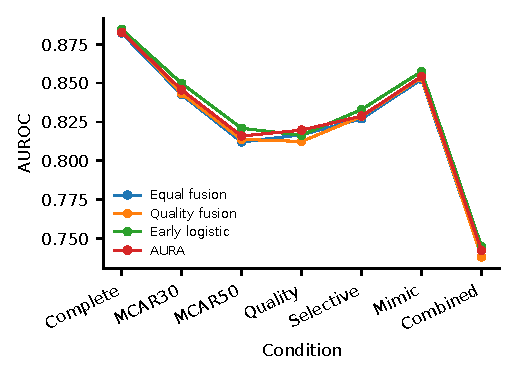
\includegraphics[width=\columnwidth]{revision_figures/robustness.pdf}
\caption{Mean AUROC across stress conditions, with labels matching the scenario table.}
\label{fig:robust}
\end{figure}
\subsection{Expert performance and attribution stability}
\begin{table}[t]
\caption{Expert performance on available records, raw $\rightarrow$ separately recalibrated Brier/ECE. Cohorts differ by availability.}
\label{tab:expert}
\centering\footnotesize
\begin{tabular}{@{}lrrrr@{}}\toprule
Expert & AUROC & AUPRC & Brier (raw/cal) & ECE (raw/cal)\\\midrule
Clinical & 0.7349 & 0.5994 & 0.195/0.196 & 0.067/0.070\\
Laboratory & 0.7693 & 0.6575 & 0.185/0.186 & 0.067/0.069\\
Imaging & 0.7541 & 0.6393 & 0.193/0.193 & 0.077/0.079\\\bottomrule
\end{tabular}
\end{table}
The laboratory expert has the highest mean AUROC on its available records; populations differ across expert availability, so the values are not a controlled modality comparison. Separate expert recalibration does not uniformly improve Brier or ECE under shift. Across all default test conditions, assertions verify normalized weights, zero weights for unavailable modalities and finite predictions. Partition disjointness and exact coalition reconstruction (tolerance $10^{-9}$) are checked, as is first-member logit reconstruction. On the fixed 150-record complete-condition anchor, pairwise mean absolute difference in coalition probability attributions is 0.02143; sign agreement is 97.15\% and largest absolute modality agreement is 90.21\%. For first-member feature-logit attributions, mean absolute differences are 0.04787, 0.05452 and 0.05480 for clinical, laboratory and imaging groups; top-feature agreement is 66.07\%, 91.29\% and 90.10\%, respectively. The anchor experiment measures stability across independent simulator-trained models at fixed inputs, not stability to missingness or clinical explanation fidelity. It does not validate user comprehension, causal effects, clinical usefulness, or the entire ensemble's feature-level explanations.
\section{Discussion and Limitations}
\subsection{Interpretation}
The central result is a limit on the methodological claim: a learned ranker improves integrated risk for late fusion, but weighted dispersion contributes no clearly established additional benefit after matching confidence, quality and availability. The sensitivity and permutation checks do not overturn that finding. A simple early-fusion logistic classifier has the best macro discrimination and lowest mean matched AURC, although the shared full-ranker contrast is inconclusive. The gate's small gains against equal and quality weighting are supported by paired intervals, but are not evidence of clinical importance. Algebraic attribution and anchor stability checks characterize model behavior only.

One explanation for the weak disagreement effect is redundancy: entropy and estimated quality already encode some of the ambiguity associated with conflicting predictions. Another is that the chosen weighted variance suppresses disagreement with low-weight modalities, even if the dissenting modality is informative. Neither hypothesis is tested directly. Alternatives include pairwise disagreement conditioned on modality identity, explicit correlation-aware fusion, and asymmetric error models. Such alternatives should be compared on untouched datasets rather than tuned against these results.
\subsection{Validity and clinical translation}
The generated class and observations are illustrative abstractions. Numerical coefficients, prevalence, mimic distributions, quality proxies and missingness mechanisms are not estimated from patients. All data therefore share a limited model of the world. The simulated negative class does not separately represent infectious sacroiliitis, mechanical pain or other diseases, and the study cannot demonstrate differential diagnosis between these categories. The simulated quality score is conveniently observable and correlated with noise; actual measurement quality may be latent, reader-dependent or confounded with severity. The selective acquisition process may encode diagnosis-related information in missingness; transfer across institutions could reverse that association.

The five-way partition and repeated seeds limit leakage within the benchmark, but the same generative family is used throughout. Calibration on the reference distribution is not a guarantee under shift. Error scores are fitted on a limited development split; the fixed threshold is selected on that same split. No formal coverage guarantee, clinical safety constraint, subgroup fairness analysis, clinician evaluation or external validation is established. No raw MRI features, real measurement units or clinical reference adjudication are available. All classifiers receive matched ranking protocols, but the auxiliary experts used for the shared context add computational cost, and this protocol does not exhaust classifier-specific uncertainty methods. Sensitivity analyses are one-factor-at-a-time and reuse the original simulator; they cannot exclude interactions or establish equivalence. The added comparisons were motivated by review and remain exploratory, not prospectively preregistered. The comparison excludes many advanced architectures, including the published evidential methods, and therefore cannot establish state-of-the-art performance. This is a lightweight exploratory study with no preregistration.

For clinical translation, an ethically governed, multicenter inception cohort with chronic back pain, matched timestamped features and independently assessed longitudinal diagnoses would be needed. A locked model should be externally evaluated against specialist assessment with subgroup reporting, calibrated predictions, false-negative costs, referral impact and clinically justified thresholds. AURA must not be used to rule out disease, recommend treatment or triage patients. TRIPOD+AI and PROBAST+AI \cite{tripod,probast} provide useful reporting and risk-of-bias considerations; this synthetic study does not constitute compliance certification.
\section{Conclusion}
In an axSpA-inspired synthetic benchmark, reliability weighting produces small paired improvements over simple late fusion, and learned error ranking can improve integrated selective risk. The additional weighted disagreement statistic does not show a clearly established benefit under matched ablation or nine sensitivity settings. A simple early logistic model remains a strong control. These results are a negative methodological finding within an illustrative generator, not evidence about real axSpA diagnostic relationships or clinical effectiveness. Independent clinical data, validated quality measures and external evaluation would be necessary for any clinical claim.
\section*{Data and Code Availability}
The accompanying source package includes the deterministic generator, original and revision experiment scripts, table/figure generation script, one generated population, per-seed metrics, sensitivity, permutation and attribution-stability files, audit files and literature matrix. All synthetic populations can be regenerated without external data. No patient data were accessed. No clinical ethics approval is claimed for this computational simulation; institutional requirements should be checked before any subsequent human-data study.
\section*{Acknowledgment}
OpenAI ChatGPT (GPT-6.2) was used to assist literature discovery and synthesis, design and implementation of the synthetic benchmark, generation of analysis code and figures, and manuscript drafting and editing. GPT-6.2 was the identified model for this revision; the underlying deployment snapshot is not independently verifiable. AI assistance included the text throughout the manuscript, figures, tables and research code, not merely language editing. Human authors retain full responsibility for verifying references, code, clinical assumptions, numerical results and conclusions and for approving the submitted work.
\begin{thebibliography}{00}
\bibitem{nice} National Institute for Health and Care Excellence, ``Spondyloarthritis in over 16s: diagnosis and management,'' NICE guideline NG65, 2017. [Online]. Available: \url{https://www.nice.org.uk/guidance/ng65}
\bibitem{mri} T. Diekhoff, R. Lambert, and K. G. Hermann, ``MRI in axial spondyloarthritis: understanding an `ASAS-positive MRI' and the ASAS classification criteria,'' 2022. [Online]. Available: \url{https://pmc.ncbi.nlm.nih.gov/articles/PMC9283193/}
\bibitem{asas} M. Rudwaleit \emph{et al.}, ``The development of Assessment of SpondyloArthritis international Society classification criteria for axial spondyloarthritis (part II): validation and final selection,'' \emph{Ann. Rheum. Dis.}, vol. 68, pp. 777--783, 2009, doi: 10.1136/ard.2009.108233.
\bibitem{adams} L. C. Adams, K. K. Bressem, and D. Poddubnyy, ``Artificial intelligence and machine learning in axial spondyloarthritis,'' \emph{Curr. Opin. Rheumatol.}, 2024, doi: 10.1097/BOR.0000000000001015.
\bibitem{meta} D. Rosillon, M. de Hooge, T. Van Den Berghe, G. Varkas, and E. Gvozdenovic, ``Performance of artificial intelligence tools in axial spondyloarthritis imaging assessment: A systematic literature review and meta-analysis,'' \emph{Joint Bone Spine}, 2026, doi: 10.1016/j.jbspin.2026.106036.
\bibitem{xie} Z. Xie \emph{et al.}, ``Enhanced diagnosis of axial spondyloarthritis using machine learning with sacroiliac joint MRI: a multicenter study,'' \emph{Insights Imaging}, vol. 16, art. 91, 2025, doi: 10.1186/s13244-025-01967-x.
\bibitem{rf} I. Redeker \emph{et al.}, ``Identification of a machine learning-based diagnostic model for axial spondyloarthritis in rheumatological routine care using a random forest approach,'' \emph{RMD Open}, vol. 10, e004702, 2024, doi: 10.1136/rmdopen-2024-004702.
\bibitem{tabnet} Z. Zhang \emph{et al.}, ``The TabNet model for diagnosing axial spondyloarthritis using MRI imaging findings and clinical risk factors,'' \emph{Int. J. Rheum. Dis.}, vol. 27, e70004, 2024, doi: 10.1111/1756-185X.70004.
\bibitem{cdss} F. Tarakci, I. A. Ozkan, M. Dogan, H. Ozer, D. Tezcan, and S. Yilmaz, ``A comprehensive clinical decision support system for the early diagnosis of axial spondyloarthritis: Multi-sequence MRI, clinical risk integration, and explainable segmentation,'' \emph{Diagnostics}, vol. 16, art. 1037, 2026, doi: 10.3390/diagnostics16071037.
\bibitem{tmc} Z. Han, C. Zhang, H. Fu, and J. T. Zhou, ``Trusted multi-view classification with dynamic evidential fusion,'' \emph{IEEE Trans. Pattern Anal. Mach. Intell.}, 2023, doi: 10.1109/TPAMI.2022.3171983.
\bibitem{qamoe} L. Sun and V. S. Sheng, ``QA-MoE: Quality-aware and stable multimodal mixture-of-experts for robust clinical prediction in noisy and missing-modal settings,'' in \emph{Proc. IJCAI}, 2026, pp. 6886--6894, doi: 10.24963/ijcai.2026/766.
\bibitem{aemrl} Y. Han, K. Zhang, X. Wang, Z. Pan, Z. Liu, and J. He, ``Trust, but verify: Uncertainty-driven evidential multimodal representation learning,'' in \emph{Proc. IJCAI}, 2026, pp. 1143--1151, doi: 10.24963/ijcai.2026/128.
\bibitem{clinical} J. A. Walsh and M. Magrey, ``Clinical manifestations and diagnosis of axial spondyloarthritis,'' \emph{J. Clin. Rheumatol.}, vol. 27, no. 8, pp. e547--e560, 2021, doi: 10.1097/RHU.0000000000001575.
\bibitem{negative} Z. Lu \emph{et al.}, ``Artificial intelligence improves the diagnosis of human leukocyte antigen (HLA)-B27-negative axial spondyloarthritis based on multi-sequence magnetic resonance imaging and clinical features,'' \emph{Quant. Imaging Med. Surg.}, 2024, doi: 10.21037/qims-24-729.
\bibitem{bal} T. Baltru\v{s}aitis, C. Ahuja, and L.-P. Morency, ``Multimodal machine learning: A survey and taxonomy,'' \emph{IEEE Trans. Pattern Anal. Mach. Intell.}, vol. 41, no. 2, pp. 423--443, 2019, doi: 10.1109/TPAMI.2018.2798607.
\bibitem{moddrop} N. Neverova \emph{et al.}, ``ModDrop: Adaptive multi-modal gesture recognition,'' \emph{IEEE Trans. Pattern Anal. Mach. Intell.}, 2016, doi: 10.1109/TPAMI.2015.2461544.
\bibitem{hemis} M. Havaei, N. Guizard, N. Chapados, and Y. Bengio, ``HeMIS: Hetero-modal image segmentation,'' 2016, arXiv:1607.05194.
\bibitem{attention} J. Liu, D. Capurro, A. N. Nguyen, and K. Verspoor, ``Attention-based multimodal fusion with contrast for robust clinical prediction in the face of missing modalities,'' \emph{J. Biomed. Inform.}, vol. 145, art. 104466, 2023, doi: 10.1016/j.jbi.2023.104466.
\bibitem{missingreview} Z. Xu, T. Zhang, and Y. Gu, ``Missing-modality robustness in clinical multimodal prediction: A mechanism-level review,'' \emph{Big Data Cogn. Comput.}, vol. 10, art. 367, 2026, doi: 10.3390/bdcc10110367.
\bibitem{dynamics} Z. Han, F. Yang, J. Huang, C. Zhang, and J. Yao, ``Multimodal dynamics: Dynamical fusion for trustworthy multimodal classification,'' in \emph{Proc. CVPR}, 2022.
\bibitem{selective} Y. Geifman and R. El-Yaniv, ``Selective classification for deep neural networks,'' in \emph{Adv. Neural Inf. Process. Syst.}, 2017.
\bibitem{guo} C. Guo, G. Pleiss, Y. Sun, and K. Q. Weinberger, ``On calibration of modern neural networks,'' in \emph{Proc. ICML}, PMLR, vol. 70, pp. 1321--1330, 2017.
\bibitem{ensembles} B. Lakshminarayanan, A. Pritzel, and C. Blundell, ``Simple and scalable predictive uncertainty estimation using deep ensembles,'' in \emph{Adv. Neural Inf. Process. Syst.}, 2017.
\bibitem{ovadia} Y. Ovadia \emph{et al.}, ``Can you trust your model's uncertainty? Evaluating predictive uncertainty under dataset shift,'' in \emph{Adv. Neural Inf. Process. Syst.}, 2019.
\bibitem{lopez} L. J. L. Lopez, F. E. Shamout, and T. G. J. Rudner, ``An empirical analysis of calibration and selective prediction in multimodal clinical condition classification,'' in \emph{Proc. Health, Inference, and Learning}, PMLR, vol. 333, pp. 794--833, 2026.
\bibitem{shap} S. M. Lundberg and S.-I. Lee, ``A unified approach to interpreting model predictions,'' in \emph{Adv. Neural Inf. Process. Syst.}, 2017.
\bibitem{desir} ``Diagnosis challenges in inception cohorts in axial spondyloarthritis: the case of the French national DESIR cohort,'' \emph{RMD Open}, vol. 10, e004484, 2024, doi: 10.1136/rmdopen-2024-004484.
\bibitem{tripod} G. S. Collins \emph{et al.}, ``TRIPOD+AI statement: updated guidance for reporting clinical prediction models that use regression or machine learning methods,'' \emph{BMJ}, vol. 385, e078378, 2024, doi: 10.1136/bmj-2023-078378.
\bibitem{probast} K. G. M. Moons \emph{et al.}, ``PROBAST+AI: an updated quality, risk of bias, and applicability assessment tool for prediction models using regression or artificial intelligence methods,'' \emph{BMJ}, vol. 388, e082505, 2025, doi: 10.1136/bmj-2024-082505.
\end{thebibliography}
\end{document}
